\documentclass{article}

\usepackage{fancyhdr}
\usepackage{extramarks}
\usepackage{minted}
\usepackage[T1]{fontenc}
\usepackage{graphicx}
\usepackage{inconsolata}
\usepackage{multicol}
\usepackage{enumitem}
\usepackage{tikz}
\usetikzlibrary{positioning}

\tikzset{
  gray box/.style={
    fill=gray!20,
    draw=gray,
    minimum width={2*#1ex},
    minimum height={2em},
  },
  annotation/.style={
    anchor=north,
  }
}


%
% Basic Document Settings
%

\topmargin=-0.45in
\evensidemargin=0in
\oddsidemargin=0in
\textwidth=6.5in
\textheight=9.0in
\headsep=0.25in

\linespread{1.1}

\pagestyle{fancy}
\lhead{\hmwkAuthorName}
\chead{\hmwkClass: \hmwkTitle}
\rhead{\firstxmark}
\lfoot{\lastxmark}
\cfoot{\thepage}

\renewcommand\headrulewidth{0.4pt}
\renewcommand\footrulewidth{0.4pt}

\setlength\parindent{0pt}

%
% Create Problem Sections
%

\newcommand{\enterProblemHeader}[1]{
\nobreak\extramarks{}{Problem \arabic{#1} continued on next page\ldots}\nobreak{}
\nobreak\extramarks{Problem \arabic{#1} (continued)}{Problem \arabic{#1} continued on next page\ldots}\nobreak{}
}

\newcommand{\exitProblemHeader}[1]{
\nobreak\extramarks{Problem \arabic{#1} (continued)}{Problem \arabic{#1} continued on next page\ldots}\nobreak{}
\stepcounter{#1}
\nobreak\extramarks{Problem \arabic{#1}}{}\nobreak{}
}

\setcounter{secnumdepth}{0}
\newcounter{partCounter}
\newcounter{homeworkProblemCounter}
\setcounter{homeworkProblemCounter}{1}
\nobreak\extramarks{Problem \arabic{homeworkProblemCounter}}{}\nobreak{}

%
% Homework Problem Environment
%
% This environment takes an optional argument. When given, it will adjust the
% problem counter. This is useful for when the problems given for your
% assignment aren't sequential. See the last 3 problems of this template for an
% example.
%
\newenvironment{homeworkProblem}[1][-1]{
\ifnum#1>0
\setcounter{homeworkProblemCounter}{#1}
\fi
\section{Problem \arabic{homeworkProblemCounter}}
\setcounter{partCounter}{1}
\enterProblemHeader{homeworkProblemCounter}
}{
\exitProblemHeader{homeworkProblemCounter}
}

%
% Homework Details
%   - Title
%   - Due date
%   - Class
%   - Section/Time
%   - Instructor
%   - Author
%

\newcommand{\hmwkTitle}{Homework\ \#4}
\newcommand{\hmwkDueDate}{March 1, 2016}
\newcommand{\hmwkClass}{Operating Systems}
\newcommand{\hmwkClassTime}{Monday \& Wednesday 3:30pm --- 5:17pm}
\newcommand{\hmwkClassInstructor}{Professor Qu}
\newcommand{\hmwkAuthorName}{Nicholas Land}

%
% Title Page
%

\title{
\vspace{2in}
\textmd{\textbf{\hmwkClass:\ \hmwkTitle}}\\
\normalsize\vspace{0.1in}\small{Due\ on\ \hmwkDueDate\ at 11:59pm}\\
\vspace{0.1in}\large{\textit{\hmwkClassInstructor\ \\ \hmwkClassTime}}
\vspace{3in}
}

\author{\textbf{\hmwkAuthorName}}
\date{}

\renewcommand{\part}[1]{\textbf{\large Part \Alph{partCounter}}\stepcounter{partCounter}\\}

%
% Various Helper Commands
%

% Alias for the Solution section header
\newcommand{\solution}{\textsc{\textbf Solution}\\}

\begin{document}

  \maketitle

  \pagebreak

  \begin{homeworkProblem}

    Consider the following process arrival list:

    \begin{center}
      \begin{tabular}{c c c}
        \underline{Name} & \underline{Arrival time} & \underline{Service time} \\
        A & $0$ & $4$ \\
        B & $3$ & $9$ \\
        C & $5$ & $2$ \\
        D & $7$ & $5$ \\
        E & $11$ & $3$ \\
        F & $13$ & $1$ \\
        G & $21$ & $4$ \\
      \end{tabular}
    \end{center}

    Consider the following scheduling methods:

    \begin{multicols}{2}
      \begin{enumerate}[label=(\alph*)]
        \item First-come first-served (FCFS)
        \item Shortest-job first (SJF)
        \vfill
        \columnbreak
        \item Shortest remaining time first (SRTF)
        \item Round-robin (RR), quantum = 5
      \end{enumerate}
    \end{multicols}

    Draw a Gantt chart (time line) showing which process is executing over time and calculate the average waiting time and average completion time. \\

    Notes : (1) In SRTF, if a process arrives with service time equal to the remaining service time of the process currently being served, the current process is not interrupted. (2) In RR, if a process arrives at the same time a quantum finishes, the running process is preempted and the new arrival executes.  The preempted process goes to the end of the ready queue. (3) Waiting time and completion time is defined as in the slides. \\

    \solution

    \begin{center}
      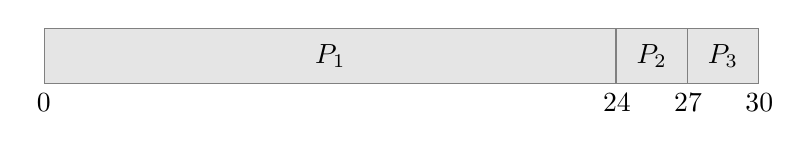
\begin{tikzpicture}[node distance=-0.5pt]
        \node [gray box=24] (p1) {\(P_{1}\)};
        \node [gray box=3, right=of p1] (p2) {\(P_{2}\)};
        \node [gray box=3, right=of p2] (p3) {\(P_{3}\)};

        \node [annotation] at (p1.south west) {0};
        \node [annotation] at (p1.south east) {24};
        \node [annotation] at (p2.south east) {27};
        \node [annotation] at (p3.south east) {30};
      \end{tikzpicture}
    \end{center}
  \end{homeworkProblem}

\end{document}
